\documentclass[10pt,twocolumn]{IEEEtran}
% replace the keyword "twocolumn" by "onecolumn" if you want a single column document

% ------------------------------------------------------------------------------------
% If you are using *TeXnicCenter*, already configured with profiles as "LaTeX -> PDF",
% do the following to create a project and have the compile hotkey Ctrl+F5:
%     Project -> Create with active file as the main file
% Do not forget to select "Uses BibTeX"
% ------------------------------------------------------------------------------------

% some useful packages:
\usepackage{graphicx}
\graphicspath{{./}{./figs/}{../figs/}{../figs/w12/}} % share figs using ../figs/
\usepackage{url}
\usepackage{amsmath}

\begin{document}

\title{}
\author{Jose Pedro Gomes}

\maketitle

\begin{abstract}
    Documentation on how the characterization of the time taken to commute between frames and events was done.
\end{abstract}

\section{Introduction}

The DVS240 camera being used allows the capture and events, but only one at a time. During runtime, it is possible to switch between the two at any time, though this takes a non-negligible amount of time. In this experiment we try to measure exactly how long it takes to switch between modes.


\section{Method}

The ROS rpg\textunderscore dvs\textunderscore ros was used to acquire data from the camera, and to perform the switch between modes.

Furthermore, a stepper motor with a wooden board attached to the shaft was used, in a clock-like mechanism. The stepper rotated at a frequency of 0.4\,Hz (2.5\,s per revolution). Fig.\,\ref{fig:w11_setup} illustrates the setup used.

\begin{figure}[ht]
    \centering
    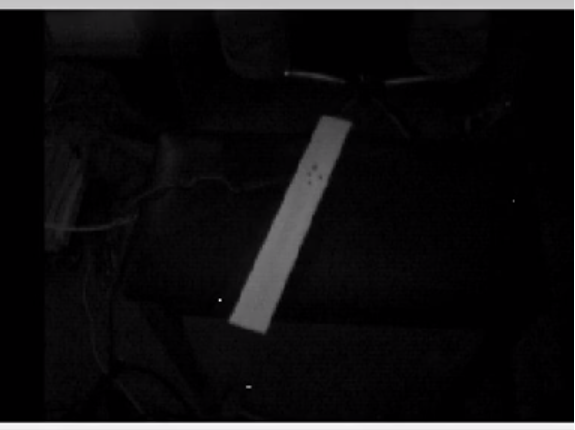
\includegraphics[width = 0.8\linewidth]{setup.png}
    \caption{Setup usedm showing a rotating wood bar attached to a stepper motor}
    \label{fig:w11_setup}
\end{figure}

A continuous stream of data was captured, switching between events and frames with no fixed interval. For each time the mode switched, the angle between the last event line and the first frame was compared (and vice-versa, when switching from frames to events), and the time elapsed was computed using \eqref{eq:w11_angle}.

\begin{equation}
    \label{eq:w11_angle}
    \text{time} = \frac{\text{angle}}{\text{freq}} = \frac{\text{angle}}{0.4}
\end{equation}

\section{Results}

Using this approach, the average angle measured switching from frames to events was between 60-70\,$^{\circ}$. This results in a latency of around 0.5\,s. 

The switch between frames and events was not measurable with this method, as the switch in this case was seamless. 

A strange artefact is worth noting, however. The first image captured was always a bright (full white) image (Fig.\,\ref{fig:w11_first}), with very little detail. It is not clear whether this is always the case because of insufficient exposure or because of the auto-focus adjusting. Nevertheless, this has to be taken into account when relying on this switch.

\begin{figure}[ht]
    \centering
    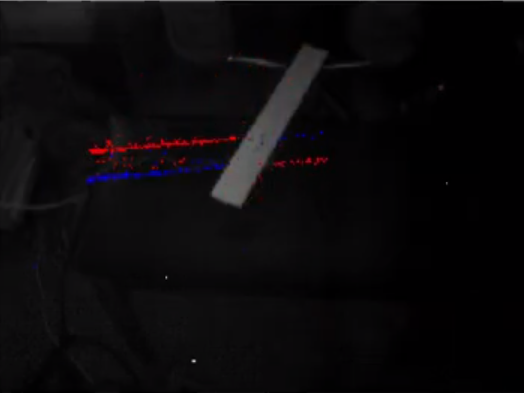
\includegraphics[width = 0.8\linewidth]{overlap.png}
    \caption{Overlaping image of frame and events, showing the elapsed time indirectly through the bar angle between the two modes}
    \label{fig:w11_setup}
\end{figure}

\begin{figure}[ht]
    \centering
    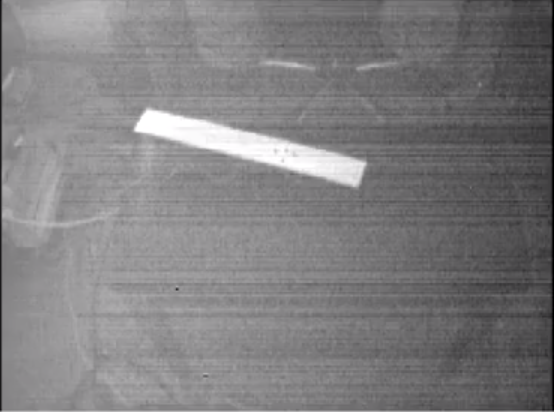
\includegraphics[width = 0.8\linewidth]{first.png}
    \caption{First frame after switching, with low quality and very bright overall}
    \label{fig:w11_first}
\end{figure}

%\bibliographystyle{plain}
%\bibliography{../thesis/ref}
% replace "project" by "thesis" if you are doing the thesis

\end{document}
